\documentclass[submission,copyright,creativecommons]{eptcs}
\providecommand{\event}{TTC 2015}
\usepackage{breakurl} % Not needed if you use pdflatex only.

% TTC additions
\usepackage{graphicx}
\usepackage{subcaption}
\usepackage{xspace}
\usepackage{rotating,amsmath,amsfonts,amssymb}
\usepackage[T1]{fontenc}
\usepackage[utf8]{inputenc}
\usepackage{todonotes}
\usepackage{float}
\usepackage{xcolor}
\usepackage{listings}
\usepackage{framed}
\usepackage{xfrac}
\usepackage{placeins}
\usepackage{paralist}
\usepackage{wrapfig}

\sloppy
% custom commands
\definecolor{negcolor}{RGB}{223,49,35}
\definecolor{newcolor}{RGB}{43,183,47}
\definecolor{delcolor}{RGB}{59,66,161}
\newcommand{\tb}{Train Benchmark\xspace}
\newcommand{\union}{\cup}
\newcommand{\tuple}[1]{\langle #1 \rangle}
\newcommand{\intersection}{\cap}
\newcommand{\parentheses}[1]{\left(#1\right)}
\newcommand{\op}[2]{\mathrm{#1}\parentheses{#2}}
\newcommand{\figref}[1]{\autoref{fig:#1}}
\newcommand{\lstref}[1]{\autoref{lst:#1}}
\newcommand{\naturaljoin}{\bowtie}
\newcommand{\antijoin}{\, \triangleright \,}
\newcommand{\eiq}{\textsc{EMF-IncQuery}}
\newcommand{\iqd}{\textsc{IncQuery-D}}
\renewcommand{\sectionautorefname}{Section}
\renewcommand{\subsectionautorefname}{Section}
\renewcommand{\subsubsectionautorefname}{Section}

\setlength{\parskip}{0em}

\newcommand{\ttcfig}[2]{
\begin{figure}[htb] 
	\centering
	\includegraphics[width=0.8\textwidth]{figures/#1}
	\caption{#2.}
	\vspace{-1em}
	\label{fig:#1}
\end{figure}}

\newcommand{\ttctransformation}[2]{
	\begin{wrapfigure}{r}{7cm}
		\centering
		\vspace{-1em}
		\includegraphics[scale=0.22]{figures/transformation-#1}
		\vspace{-1em}
		\footnotesize
		\begin{align*}
		\sf #2
		\end{align*}
		\vspace{-3em}
	\end{wrapfigure}
}

\newcommand{\ttcfigscale}[3]{
\begin{figure}[htb]
	\centering
	\includegraphics[scale=#3]{figures/#1}
	\caption{#2.}
	\label{fig:#1}
\end{figure}}

\definecolor{lightgray}{rgb}{0.95,0.95,0.95}
\lstset{
	basicstyle=\scriptsize\ttfamily, % print whole listing small
	keywordstyle=\color{black}\bfseries, % bold black keywords
	identifierstyle=, % nothing happens
	commentstyle=\color{green}, % green comments
	stringstyle=\scriptsize,
	showstringspaces=false, % no special string spaces
	aboveskip=3pt,
	belowskip=3pt,
	backgroundcolor=\color{lightgray},
	columns=flexible,
	keepspaces=true
} 

% metadata
\title{The TTC 2015 \tb Case\\ for Incremental Model Validation\thanks{This work was partially supported by the MONDO (EU ICT-611125) project and Red Hat Inc.}}
\author{G\'{a}bor Sz\'{a}rnyas \qquad Oszk\'{a}r Semer\'{a}th \qquad Istv\'{a}n R\'{a}th \qquad D\'{a}niel Varr\'{o}
\institute{Budapest University of Technology and Economics\\
Department of Measurement and Information Systems\\
H-1117 Magyar tud\'{o}sok krt. 2, Budapest, Hungary}
\email{\{szarnyas, semerath, rath, varro\}@mit.bme.hu}
}
\def\titlerunning{The TTC 2015 \tb Case for Incremental Model Validation}
\def\authorrunning{G. Sz\'{a}rnyas et al.}

\begin{document}
\maketitle

\begin{abstract}
In model-driven development of safety-critical systems (like automotive, avionics or railways), well-formedness of models is repeatedly validated in order to detect design flaws as early as possible. Validation rules are often implemented by a large amount of imperative model traversal code which makes those rule implementations complicated and hard to maintain. Additionally as models are rapidly increasing in size and complexity, efficient execution of these operations is challenging for the currently available toolchains. However, checking well-formedness constraints can be interpreted as evaluation of model queries, and the operations as model transformations, where the validation task can be specified in a concise way, and executed efficiently.

This paper presents a benchmark case and an evaluation framework to systematically assess the scalability of validating and revalidating well-formedness constraints over large models. The benchmark case defines a typical well-formedness validation scenario in the railway domain including the metamodel, an instance model generator, and a set of well-formedness constraints captured by queries and repair operations (imitating the work of systems engineers by model transformations). The benchmark case focuses on the execution time of the query evaluations with a special emphasis on reevaluations, as well as simple repair transformations.
\end{abstract}

\section{Introduction}

During the development of safety critical software like automotive, avionics or train control systems, different kind of models are frequently used. The goal of this approach is to develop models to assist the automated generation of various design artifacts (source code, configuration files, etc.) However, design errors of the system model invalidate the correctness of the generated artifacts, thus it is critical to check the well-formedness of such models. Additionally, it is considerably more expensive to fix design flaws in the later stage of the development, thus it is important to detect them as soon as possible by checking the well-formedness constraints repeatedly.

Model validation problems are often addressed by model transformation engines: error cases are defined by model queries, the results of which can be automatically repaired by transformation steps. In practice, this is challenging due to two factors: (i) \emph{instance model sizes} are exhibiting a tremendous growth as the complexity of systems-under-design is increasing, (ii) the \emph{sophistication of validation constraints} in toolchains is increasing. As a consequence, validation of industrial models is challenging or may become completely unfeasible.

To address this challenge, the \tb is a macro benchmark that aims to measure repetitive query evaluation performance. While there are a number of existing benchmarks for queries over relational databases%~\cite{TPC-C, Wisconsin} 
and triplestores, %~\cite{BSBM, SP2Bench, DBpedia, LUBM}, 
modeling tool workloads for well-formedness constraint validation are significantly different~\cite{ase2013}. Specifically, modeling tools use much more complex queries than typical transactional systems, and the real world performance is more affected by response time (i.e.\ execution time for a specific operation such as validation or transformation) rather than throughput (i.e.\ the number of parallel transactions). Also, previous TTC cases did not focus on measuring the performance of query reevaluation.

%The \tb defines a scenario that is specifically modeled after \emph{model validation} in (domain-specific) modeling tools: at first, the entire model is validated, then each model transformation is followed by an immediate revalidation. The primary goal of the benchmark is to measure the execution time of each phase. The benchmark uses a domain-specific model of a railway system that originates from the \mbox{MOGENTES} EU FP7~\cite{MOGENTES} project, where both the metamodel and the well-formedness rules were defined by railway domain experts. Some of the queries are in close correspondence with constraints in the AUTOSAR standard~\cite{AUTOSAR}. 

The source code is available at \url{https://github.com/FTSRG/trainbenchmark-ttc}. This case is strongly based on the \tb~\cite{TrainBenchmarkTechReport}, an ongoing benchmark project of our research group. %~\cite{bigmde2013, ase2013, bigmde2014, models2014, scp2015}.

\section{Case Description}

A \emph{benchmark case} configuration in the \tb consists of an \emph{instance model} (\autoref{instancemodels}), a \emph{query} and a \emph{repair transformation} (\autoref{tasks}) describing constraint violating elements. As a result of a benchmark case run, the \emph{execution times} of each phase, the \emph{memory usage} and the \emph{number of invalid elements} are measured and recorded. The number of invalid elements are used to check the correctness of the validation, however the collection of element identifiers must also be available for later processing.

\subsection{Metamodel}

The metamodel of the \tb is shown in~\figref{metamodel}. A train \textsf{route} is defined by a sequence of \textsf{sensor}s. Sensors are associated with \textsf{track elements} which are either \textsf{segment}s (with a specific length) or \textsf{switch}es. A route follows certain \textsf{switch positions} which describe the \emph{required} state of a switch belonging to the route. Different route definitions can specify different states for a specific switch. Each route has a \textsf{semaphore} on its entry and exit. \figref{railway} shows a typical railway network.

Every railway element is a subtype of the class \textsf{RailwayElement} which has a unique identifier (\textsf{id}). The root of the model is a \textsf{RailwayContainer} which contains the semaphores and the routes of the model. Additionally, the railway container has an \textsf{invalids} reference for storing elements. This is used for serializing EMF models (\autoref{emf-models}). 

\ttcfig{railway}{Illustration for the concepts in the \tb models}

\subsection{Instance Models}
\label{instancemodels}

The instance models are systematically generated for the metamodel: small model fragments are created and connected to each other. Based on the model queries, the generator injects errors to the model by removing edges and changing attribute values with a certain probability. The probability of injecting an error to violate a pattern (\autoref{tasks}) is shown in~\autoref{tab:errorpercentages}.

This generation method controls the number of matches of all defined model queries. To avoid highly symmetric models, the exact number of elements and cardinalities are randomized. This brings artificially generated models closer to real world instances and prevents query tools from abusing the artificial regularity of the model.  To assess scalability, the benchmark uses instance models of growing sizes, each model containing twice as many model elements as the previous one. The instance models are designated by powers of two (1, 2, 4, 8, \ldots), the smallest model containing about 5000 model elements. 

\subsection{Benchmark Phases}
\label{sec:phases}

\ttcfig{benchmark-phases}{Phases of the benchmark}

To simulate a typical validation workload, four \emph{phases} were defined (\figref{benchmark-phases}).

\begin{compactenum}
	\item During the \textsf{read} phase, the instance model is loaded from hard drive to memory. This includes the parsing of the input as well as initializing data structures (e.g.\ indexes) of the tool.
	\item In the \textsf{check} phase, the instance model is queried to identify invalid elements. The result of this phase is a set of the invalid elements, which will be used in the next phase.
	\item In the \textsf{repair} phase, the model is changed to simulate the effects (and measure the performance) of model modifying operations. The transformations are always performed on a subset of the model elements returned by the \textsf{check} phase.
	\item The revalidation of the model is carried out in the \textsf{recheck} phase similarly to the \textsf{check} phase. In real-world scenarios, there are often multiple transformations in the system which may interfere with the results of the query. Because of this, we require the tools to reevaluate the query with regards to the current state of the model.
\end{compactenum}

The repair operation intends to fix invalid models elements based on the invalid objects identified during the previous \textsf{check} or \textsf{recheck} phase. We defined two strategies to determine the size of the change set:

\begin{compactdesc}
\item[fixed] 10 of invalid model elements is modified. This tests the efficiency of handling small change sets.
\item[proportional] 10\% of the dresult set is modified. This tests the efficiency of handling large change sets.
\end{compactdesc}

\subsection{Queries}
\label{queries}

The \emph{queries} used in the validation scenario are introduced both informally and as graph patterns. In complexity, the queries range from simple attribute value checks to complex path constraints consisting of several join operations: two simple queries use at most 2 objects (\textsf{PosLength} and \textsf{SwitchSensor}) and three complex queries use 4--8 objects and multiple join operations (\textsf{RouteSensor}, \textsf{SemaphoreNeighbor}, \textsf{SwitchSet}). 

\subsubsection{Graph Patterns and Transformations}

The purpose of the queries is to check well-formedness constraints by matching graph patterns looking for errors in the model. The \emph{graph patterns} are defined by a \emph{name}, a list of symbolic object parameters and the constraints to be satisfied by the parameters. A \emph{pattern match} maps each symbolic parameter to a model object, where the mapping satisfies the conditions defined by the constraints. The result of the query is the set of all possible matches. The absence of pattern matches means that the model is well-formed, and the matches of the error pattern marks the invalid elements. The \emph{match set} contains all matches for a given pattern.

In the \emph{repair} phase, some model elements are \emph{deterministically selected} and repaired. In order to ensure \emph{repeatable results}, (1) the elements for transformation are chosen using a pseudorandom generator, (2) the elements are always selected from the deterministically sorted list (\autoref{queries}).

\section{Tasks}
\label{tasks}

For each task, we present the well-formedness constraints. The \emph{queries} are looking for violations of these constraints. We describe the meaning and the goal of each query and show a graphical notation of the associated graph pattern. We also define the matches as tuples to ensure that the ordering of the matches is consistent between the implementations (\autoref{ordering}). The \emph{repair transformations} are represented as graph transformations. For defining the patterns and transformations, we used a graphical syntax similar to GROOVE~\cite{rensink2004groove} with a couple of additions:

\begin{compactitem}
  \item Filter conditions are shown in \textit{italic} font.
  \item Negative application conditions are shown with in a \textcolor{negcolor}{red} rectangle with the \textcolor{negcolor}{\textsf{NEG}} caption.
  \item The insertions are with a \textcolor{newcolor}{\guillemotleft{}new\guillemotright{}} caption. Attribute updates are also show in \textcolor{newcolor}{green}. % while deletions are marked with a \textcolor{delcolor}{\guillemotleft{}del\guillemotright{}} caption
\end{compactitem}

\ttctransformation{poslength}{\tuple{segment}}

\paragraph{PosLength.} Every segment must have a positive length.

\noindent\textit{Query.} The query checks for segments with a length less than or equal to zero. \\
\textit{Repair transformation.} The \textsf{length} attribute of the \textsf{segment} in the match is updated to $- \mathsf{length} + 1$. \\
\textit{Goal.} This query defines an attribute check. This is a common use case in validation scenarios.


\ttctransformation{switchsensor}{\tuple{sw}}
\paragraph{SwitchSensor.} Every switch must have at least one sensor connected to it.

\noindent\textit{Query.} The query checks for switches that have no sensors associated with them. \\
\textit{Repair transformation.} A \textsf{sensor} is created and connected to the \textsf{switch}. \\
\textit{Goal.} This query checks whether an object is connected to a relation. This pattern is common in more complex queries, e.g.\ it is used in the \textsf{RouteSensor} and the \textsf{SemaphoreNeighbor} queries.


\ttctransformation{switchset}{\tuple{semaphore, route, swP, sw}}
\paragraph{SwitchSet.} The entry semaphore of a route may only show GO if all switches along the route are in the position prescribed by the route. \\
\textit{Query.} The query checks for routes which have a semaphore that show the GO signal. Additionally, the route follows a switch position (\textsf{swP}) that is connected to a switch (\textsf{sw}), but the switch position (\textsf{swP.position}) defines a different position from the current position of the switch (\textsf{sw.currentPosition}). \\
\textit{Repair transformation.} The \textsf{currentPosition} attribute of the \textsf{switch} is set to the \textsf{position} of \textsf{swP}. \\
\textit{Goal.} This pattern tests the efficiency of the join and filtering operations.

\ttctransformation{routesensor}{\tuple{route, sensor, swP, sw}}
\paragraph{RouteSensor.} All sensors that are associated with a switch that belongs to a route must also be associated directly with the same route. \\
\textit{Query.} The query looks for sensors that are connected to a switch, but the sensor and the switch are not connected to the same route. \\
%\textbf{Match.} $} \rangle$ \\
\textit{Repair transformation.} The missing \textsf{definedBy} edge is inserted by connecting the \textsf{route} in the match to the \textsf{sensor}. \\
\textit{Goal.} This pattern checks for the absence of circles, so the efficiency of the join and the antijoin operations is tested.

\ttctransformation{semaphoreneighbor}{\langle & \sf semaphore, route1, route2, \\ & \sf sensor1, sensor2, te1, te2 \rangle}
\paragraph{SemaphoreNeighbor.} Routes that are connected through sensors and track elements must belong to the same semaphore. \\
\textit{Query.} The query checks for routes (\textsf{route1}) which have an exit semaphore (\textsf{semaphore}) and a sensor (\textsf{sensor1}) connected to a track element (\textsf{te1}). This track element is connected to another track element (\textsf{te2}) which is connected to another sensor (\textsf{sensor2}) which (partially) defines another, different route (\textsf{route2}), while the semaphore is not on the entry of this route (\textsf{route2}). \\
%\ttctransformation{semaphoreneighbor}
\textit{Repair transformation.} The \textsf{route2} node is connected to the \textsf{semaphore} node with an \textsf{entry} edge. \\
\textit{Goal.} This pattern checks for the absence of circles, so the efficiency of the join operation is tested. One-way navigable references are also present in the constraint, so the efficiency of their evaluation is also measured. Subsumption inference is required, as the two track elements can be switches or segments.

\paragraph{Acknowledgements.} The authors would like to thank Benedek Izsó for originally designing and implementing the \tb, Tassilo Horn for providing valuable comments regarding both the specification of the case and the implementation of the benchmark framework, and Zsolt Kővári for his contributions in the benchmark and visualization scripts.

\bibliographystyle{eptcs}
\bibliography{ttc}

\clearpage

\appendix

\section{Metamodel}

\begin{figure}[h!]
	\centering
	\begin{subfigure}[b]{\textwidth}
		\centering
		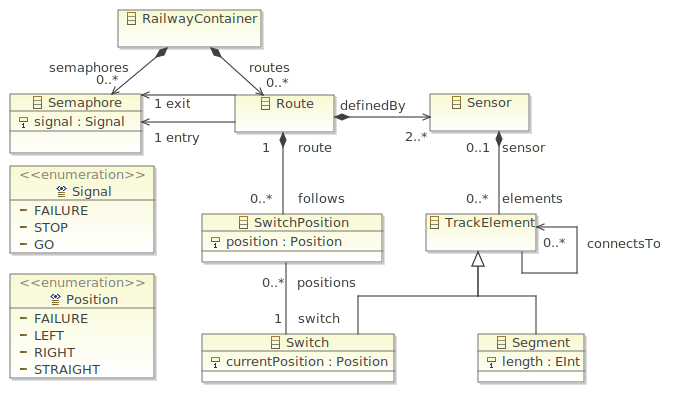
\includegraphics[scale=0.6]{figures/railway-containments}
		\caption{Containment hierarchy and references}
		\label{fig:railway-containments}
	\end{subfigure}
		\begin{subfigure}[b]{\textwidth}
			\centering
			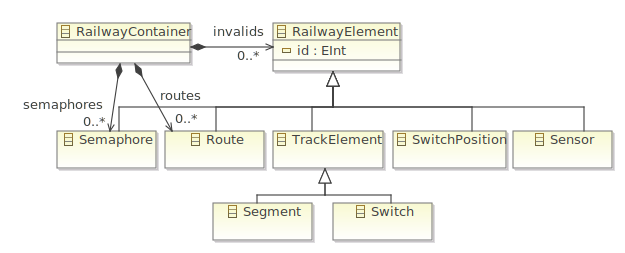
\includegraphics[scale=0.6]{figures/railway-inheritance}
			\caption{Supertype relations}
			\label{fig:railway-inheritance}
		\end{subfigure}
	\caption{The metamodel of the \tb.}
	\label{fig:metamodel}
\end{figure}

\section{Implementation}

To aid the development of case solutions, we provide a framework using predefined input and output formats, along with two reference implementations.

\subsection{Instance Model Formats}

\begin{table}
	\centering
	\begin{tabular}{ | l | c | }
		\hline
		\bf attribute / edge & \bf error percentage \\\hline
		\sf Segment.length          & 6\%  \\\hline
		\sf Route.definedBy         & 10\% \\\hline
		\sf Route.exit              & 15\% \\\hline
		\sf Switch.sensor           & 35\% \\\hline
		\sf SwitchPosition.position & 30\% \\\hline
	\end{tabular}
	\caption{Error percentages in the generated instance model.}
	\label{tab:errorpercentages}
\end{table}

\subsubsection{EMF Models}
\label{emf-models}

The EMF models are serialized to standard XMI format using the generated EMF code. The injection of errors during the instance model generation (\autoref{instancemodels}) causes some containment errors. Invalid elements violating the containment hierarchy could not be serialized. As the benchmark requires invalid models, the invalid elements are connected to the root element of the instance model by the \textsf{invalids} reference~\figref{railway-inheritance}.

\subsubsection{Non-EMF Models}

The generator defines a graph-like interface for creating the models. The EMF model generator is an implementation of this interface. To generate non-EMF models, the following approaches are recommended: (1) either create a custom class which implements the \textsf{Generator} interface or (2) generate the EMF models and convert them to another representation.

\subsection{Ordering of the Match Set}
\label{ordering}

The matches in the match set may be returned in any collection (e.g.\ a list or a set) in any order, given that the collection is unique. In order to ensure that the benchmark is \emph{repeatable}, this collection is copied to a sorted list. The sorting is carried out using by defining the ordering between matches.

To \emph{compare} matches $M_1 = \langle a_1, a_2, \ldots, a_n \rangle$ and $M_2 = \langle b_1, b_2, \ldots b_n \rangle$, we take the first elements in each match ($a_1$ and $b_1$) and compare their identifiers. If the first elements are equal, we compare the second elements ($a_2$ and $b_2$) and so on until we find two different model elements. This is guaranteed by the fact that the collection is unique, so it cannot contain two identical matches.

For example, for the \textsf{RouteSensor} query, a match set may be returned by tool $A$ as list
\[\left(
\langle\textsf{route}: 8, \textsf{sensor}: 12, \textsf{switchPosition}: 4, \textsf{sw}: 10\rangle;
\langle\textsf{route}: 5, \textsf{sensor}: 1, \textsf{switchPosition}: 13, \textsf{sw}: 7\rangle
\right)\]
and by tool $B$ as set
\[\left\{
\langle\textsf{route}: 5, \textsf{sensor}: 1, \textsf{switchPosition}: 13, \textsf{sw}: 7\rangle;
\langle\textsf{route}: 8, \textsf{sensor}: 12, \textsf{switchPosition}: 4, \textsf{sw}: 10\rangle
\right\}\]
For both implementations, the framework creates a \emph{sorted copy}, resulting in the list
\[\left(
\langle\textsf{route}: 5, \textsf{sensor}: 1, \textsf{switchPosition}: 13, \textsf{sw}: 7\rangle;
\langle\textsf{route}: 8, \textsf{sensor}: 12, \textsf{switchPosition}: 4, \textsf{sw}: 10\rangle
\right)\]
The ordered list is also used to ensure that the transformations are performed on the same model elements, regardless of the return order of the match set.

\subsection{Building the Projects}

The Train Benchmark case defines a framework and application programming interface that enables the integration of additional tools. The reference implementation contains a benchmark suite for queries implemented in Java and \eiq{}. Both the framework and the reference implementations are written in Java~7.

For building the projects, we used Apache Maven\footnote{\url{https://maven.apache.org/}}, one of the most widely used Java build systems. The build is configured so that the binaries are able to run without an Eclipse application. A significant proportion of modeling tools are integrated to the Eclipse plug-in environment. In order to support such systems, our projects also have a plug-in nature. This way, they can be integrated with Eclipse (and OSGi) plug-ins as well and can be built without Maven.

\subsection{Running the Projects}

The scripts can parametrized by a simple JSON configuration file which defines:

\begin{itemize}
	\item the range of the instance models from \texttt{minSize} to \texttt{maxSize},
	\item the list of queries specified (\autoref{queries}),
	\item the list of tools,
	\item the number of runs,
	\item the number of repair--recheck iterations,
	\item the change set strategies,
	\item the JVM arguments (e.g.\ maximum heap memory).
\end{itemize}

The default configuration is stored in the \texttt{config/config.json} file. Please use this as a basis for your configuration.

\begin{lstlisting}
{
  "MinSize": 1,
  "MaxSize": 2,
  "Queries": ["PosLength", "RouteSensor", "SwitchSensor", "SwitchSet", "SemaphoreNeighbor"],
  "Tools": [<your tool>],
  "ChangeSets": ["fixed", "proportional"],
  "Runs": 1,
  "IterationCount": 5,
  "JVM": {"vmargs": "-Xmx4G"}
}
\end{lstlisting}

\subsection{Interpreting the Output}

Measurements are automatically recorded by our benchmark framework and stored in TSV (Tab-Separated Values) format. This can be used to automatically create diagrams with the provided R\footnote{\url{https://www.r-project.org/}} script and provide comparable plots. For publishing performance results, please stick to the format generated by the framework.

\autoref{tab:exampleoutput} shows an example output. The \textsf{ChangeSet} defines the change set size (\emph{fixed} or \emph{proportional}, see~\figref{benchmark-phases}). The Train Benchmark is executed 5 times, the index of the current run is stored in the \textsf{RunIndex} attribute. The \textsf{Query} is executed by the \textsf{Tool} on the model with the given \textsf{Size}. The validation errors are repaired in multiple iterations, the index of the current iteration is shown in the \textsf{Iteration} attribute. Multiple values (\textsf{MetricValue}) of different metrics (\textsf{MetricName}) are measured during the benchmark. The execution time (\textit{time}) and memory consumption (\textit{memory}) for the \textit{read}, \textit{check}, \textit{repair} and \textit{recheck} phases are collected. The name the current phase is defined by the \textsf{PhaseName}. Additionally, the result set size (\textit{rss}) is stored for the \textit{check} phase and the iterations in the \textit{recheck} phase.


\section{Evaluation Criteria}

The solutions are checked and evaluated for functional, usability and performance aspects.

\subsection{Correctness and Completeness of Model Queries and Transformations}
The goal of the correctness check is to determine if the different model query and transformation tasks are correctly and fully implemented in the submitted solutions.
We provide the number of invalid model elements in several models detected by our reference implementation for each query and iteration step. If the result sizes are consistently equal, the solution is considered to be correct.

The expected results are available at \url{https://github.com/FTSRG/trainbenchmark-ttc/tree/master/expected-results}.

Each task is scored independently $0-3$ points by the following rules:
\begin{itemize}
	\item $\mathbf{0}$   \textbf{points:} The task is not solved.
	\item $\mathbf{1-2}$ \textbf{points:} The task is partially solved, the solution provides the subset or the superset of the expected results.
	\item $\mathbf{3}$   \textbf{points:} The task is completely and correctly solved.
	\item $\mathbf{-1}$  \textbf{point:} Only the query is implemented, but the transformation is not.
\end{itemize}

\noindent\framebox[\textwidth][c]{\textbf{Correctness and completeness:} $ 5~\textrm{tasks} \times 3~\textrm{points} = 15~\textrm{points} $}

\subsection{Conciseness}

The validation rules are frequently changed and extended, therefore it is important to be able to define queries and transformations in a concise manner. These properties are scored based on the following rules:

\begin{itemize}
	\item $\mathbf{0}$   \textbf{points:} The task is not solved.
	\item $\mathbf{1}$   \textbf{point:} The task is solved, but the solution is not significantly more concise than it would be in a general-purpose imperative language (e.g.\ Java), or the task is partially solved and the result set needs additional processing.
	\item $\mathbf{2}$   \textbf{points:} The task is solved, the query and the transformation is defined in a declarative, visual or other query language, but the specification is hard to formulate.
	\item $\mathbf{3}$   \textbf{points:} The solution is compact, the query and the transformation are defined in a concise manner.
	\item $\mathbf{-1}$  \textbf{point:} Either the query or the transformation is implemented.
\end{itemize}

\noindent\framebox[\textwidth][c]{\textbf{Conciseness:} $5~\textrm{tasks} \times 3~\textrm{points} = 15~\textrm{points}$}

\subsection{Readability}

The readability and descriptive power of each query and transformation is scored with respect to a model validation use case. The score represents how well model queries are used as model constraints, and how well repair operations can be expressed by model transformations. The score is given based on the following rules:
\begin{itemize}
	\item $\mathbf{0}$   \textbf{points:} The task is not solved.
	\item $\mathbf{1}$   \textbf{point:} The task is solved, but the solution is not significantly more readable than it would be in a general-purpose imperative language (e.g.\ Java), or the task is just partially solved. For example, a typical EMF validator should get 1 point.
	\item $\mathbf{2}$   \textbf{points:} The task is solved, the query and the transformation follows the description of the constraint and repair rule, but it is difficult to comprehend the meaning of the solution. For example, a foreign key constraint checked by a query formulated in SQL should get 2 points.
	\item $\mathbf{3}$   \textbf{points:} The solution could be presented in the documentation of the modeling domain, and it is easier to comprehend than a textual description in natural language. For example, a solution similar to the graphical notation used in this paper should get 3 points.
	\item $\mathbf{-1}$  \textbf{point:} If the language is only able to express either the constraint (e.g.\ OCL) or the repair operation.
\end{itemize}

\noindent\framebox[\textwidth][c]{\textbf{Readability:} $5~\textrm{tasks} \times 3~\textrm{points} = 15~\textrm{points}$}

\subsection{Performance on Large Models}
The goal of the performance measurements is to check the applicability of the submitted solutions on large industrial models. During the performance tests the execution times will be measured for different scenarios and increasing model sizes.

Please restrict your benchmarks to those input models that can be processed within 5 minutes or less. Runs that take longer than 5 minutes will not be considered in the evaluation. Please provide a solution that can run on an x64-based Linux system with 4+~GB of memory, and that can be started on the command-line. This will be important to reproduce your results on a remote testing system. Please document the setup of your solution and the requirements to the system environment.

We defined two validation scenarios, based on the phases defined in~\autoref{sec:phases}:

\begin{description}
	\item[batch] The model is loaded (\textsf{read}) and validated (\textsf{check}).
	\item[repeated] The model is loaded (\textsf{read}) and validated (\textsf{check}), then the model is edited (\textsf{repair}) and revalidated (\textsf{recheck}) 10 times.
\end{description}

The performance of the solutions are compared in 20 \emph{tournaments}:

\begin{itemize}
	\item The tournaments are calculated for the 5 tasks. If a solution skips a task, it is not considered in the tournament.
	\item Each solution is measured for both \emph{batch} and \emph{repeated} validation.
	\item Each solution is measured for both \emph{fixed} and \emph{proportional} change sets.
\end{itemize}

A solution gets from 0 to 1 points for a tournament which is launched for increasing model sizes. The score is based on the maximum size that the solution is able to handle, and its execution time relative to the fastest solution. Each measurement is executed 5 times and the median value is taken.

\begin{itemize}
	\item The model size is increased as long as there is a solution that is able to solve it in the given time limit. This results in \emph{rounds} $k = 1, 2, 3, \ldots, n$ for sizes $2^{k-1}$ ($1, 2, 4, \ldots, 2^{n-1}$).  
	\item For each tournament, a solution earns a score between 0 and 1, determined by
	\[\frac{\sum^{\mathit{n}}_{k=1} \mathit{score}(k)}{\sum^{\mathit{n}}_{k=1} k}, \]
	
	where
	
	\[
	\mathit{score}(k) =
	\begin{cases}
	\mathit{score}_\mathit{size}(k) \times \mathit{score}_\mathit{time}(k), & \text{if the solution runs correctly and within the given time limit,}\\
	0,                                                                      & \text{if the solution fails to run correctly or exceeds the given time limit,}
	\end{cases}
	\]
	
	and $\sum^{\mathit{n}}_{k=1} k = \mathit{n}\cdot(\mathit{n}+1)/2$ is used for normalizing the result.
	
	\item For each round $\mathit{k}$ from 1 to $n$, if a solution is able to complete the validation, it is rewarded $k$ points:
	\begin{itemize}
		\item round 1 (size 1): the winner earns 1 point,
		\item round 2 (size 2): the winner earns 2 points,
		\item round 3 (size 4): the winner earns 3 points,
		\item \ldots
		\item round $n$ (size $2^{n-1}$): the winner earns $n$ points.
	\end{itemize}
	
	The formula is specified as:
	
	\[ \mathit{score}_\mathit{size}(k)= k \]
	
	\item The fastest solution in each round earns 1 point, the other solutions earn partial points, based on the proportion of the current solution's execution time to the fastest execution time. The logarithm of this ratio for base 2 defines the score. For example:
	\begin{itemize}
		\item if a solution takes $2 \times$ as long, it earns \sfrac{1}{2} points, 
		\item if a solution takes $4 \times$ as long, it earns \sfrac{1}{3} points,
		\item if a solution takes $8 \times$ as long, it earns \sfrac{1}{4} points,
		\item and so on.
	\end{itemize}
	
	The formula is specified as:
	
	\[ \mathit{score}_\mathit{time}(k)=\frac{1}{1+\log_2\left(\frac{\text{the solution's execution time in round $k$}}{\text{the fastest execution time in the round $k$}}\right)} \]
\end{itemize}

In conclusion, a solution earns up to 20 points for \textbf{performance}:

\noindent\framebox[\textwidth][c]{$5~\textrm{tasks} \times 2~\textrm{validation scenarios} \times 2~\textrm{change set sizes } \times \textrm{up to 1 points} = 20~\textrm{points}$}

\subsection{Overall Evaluation}

The scores of each aspect of the submitted solution are summarized to derive the final score (max.\ 65 points) used for ranking the submitted solutions.

\begin{table}
\centering
\footnotesize
\begin{tabular}{| l | r | l | r | l | l | r | l | r |}
\hline
\sf ChangeSet & \sf RunIndex & \sf Tool & \sf Size & \sf Query & \sf PhaseName & \sf Iteration & \sf MetricName & \sf MetricValue\\\hline
fixed & 1 & EMFIncQuery & 1 & PosLength & check & 0 & rss & 43\\\hline
fixed & 1 & EMFIncQuery & 1 & PosLength & recheck & 1 & rss & 33\\\hline
fixed & 1 & EMFIncQuery & 1 & PosLength & recheck & 2 & rss & 23\\\hline
fixed & 1 & EMFIncQuery & 1 & PosLength & recheck & 3 & rss & 13\\\hline
fixed & 1 & EMFIncQuery & 1 & PosLength & recheck & 4 & rss & 3\\\hline
fixed & 1 & EMFIncQuery & 1 & PosLength & recheck & 5 & rss & 0\\\hline
fixed & 1 & EMFIncQuery & 1 & PosLength & recheck & 6 & rss & 0\\\hline
fixed & 1 & EMFIncQuery & 1 & PosLength & recheck & 7 & rss & 0\\\hline
fixed & 1 & EMFIncQuery & 1 & PosLength & recheck & 8 & rss & 0\\\hline
fixed & 1 & EMFIncQuery & 1 & PosLength & recheck & 9 & rss & 0\\\hline
fixed & 1 & EMFIncQuery & 1 & PosLength & recheck & 10 & rss & 0\\\hline
fixed & 1 & EMFIncQuery & 1 & PosLength & read & 0 & time & 754739233\\\hline
fixed & 1 & EMFIncQuery & 1 & PosLength & read & 0 & memory & 6711048\\\hline
fixed & 1 & EMFIncQuery & 1 & PosLength & check & 0 & time & 51752\\\hline
fixed & 1 & EMFIncQuery & 1 & PosLength & check & 0 & memory & 6582280\\\hline
fixed & 1 & EMFIncQuery & 1 & PosLength & recheck & 1 & time & 5116\\\hline
fixed & 1 & EMFIncQuery & 1 & PosLength & recheck & 1 & memory & 2848944\\\hline
fixed & 1 & EMFIncQuery & 1 & PosLength & recheck & 2 & time & 4304\\\hline
fixed & 1 & EMFIncQuery & 1 & PosLength & recheck & 2 & memory & 2823352\\\hline
fixed & 1 & EMFIncQuery & 1 & PosLength & recheck & 3 & time & 8533\\\hline
fixed & 1 & EMFIncQuery & 1 & PosLength & recheck & 3 & memory & 2798328\\\hline
fixed & 1 & EMFIncQuery & 1 & PosLength & recheck & 4 & time & 4362\\\hline
fixed & 1 & EMFIncQuery & 1 & PosLength & recheck & 4 & memory & 2781144\\\hline
fixed & 1 & EMFIncQuery & 1 & PosLength & recheck & 5 & time & 4086\\\hline
fixed & 1 & EMFIncQuery & 1 & PosLength & recheck & 5 & memory & 2780248\\\hline
fixed & 1 & EMFIncQuery & 1 & PosLength & recheck & 6 & time & 4723\\\hline
fixed & 1 & EMFIncQuery & 1 & PosLength & recheck & 6 & memory & 2780344\\\hline
fixed & 1 & EMFIncQuery & 1 & PosLength & recheck & 7 & time & 8350\\\hline
fixed & 1 & EMFIncQuery & 1 & PosLength & recheck & 7 & memory & 2780440\\\hline
fixed & 1 & EMFIncQuery & 1 & PosLength & recheck & 8 & time & 12007\\\hline
fixed & 1 & EMFIncQuery & 1 & PosLength & recheck & 8 & memory & 2780536\\\hline
fixed & 1 & EMFIncQuery & 1 & PosLength & recheck & 9 & time & 4107\\\hline
fixed & 1 & EMFIncQuery & 1 & PosLength & recheck & 9 & memory & 2780632\\\hline
fixed & 1 & EMFIncQuery & 1 & PosLength & recheck & 10 & time & 21459\\\hline
fixed & 1 & EMFIncQuery & 1 & PosLength & recheck & 10 & memory & 2780776\\\hline
fixed & 1 & EMFIncQuery & 1 & PosLength & repair & 1 & time & 2861134\\\hline
fixed & 1 & EMFIncQuery & 1 & PosLength & repair & 1 & memory & 2855192\\\hline
fixed & 1 & EMFIncQuery & 1 & PosLength & repair & 2 & time & 3558045\\\hline
fixed & 1 & EMFIncQuery & 1 & PosLength & repair & 2 & memory & 2824640\\\hline
fixed & 1 & EMFIncQuery & 1 & PosLength & repair & 3 & time & 1090021\\\hline
fixed & 1 & EMFIncQuery & 1 & PosLength & repair & 3 & memory & 2800656\\\hline
fixed & 1 & EMFIncQuery & 1 & PosLength & repair & 4 & time & 1062007\\\hline
fixed & 1 & EMFIncQuery & 1 & PosLength & repair & 4 & memory & 2781272\\\hline
fixed & 1 & EMFIncQuery & 1 & PosLength & repair & 5 & time & 1235721\\\hline
fixed & 1 & EMFIncQuery & 1 & PosLength & repair & 5 & memory & 2780336\\\hline
fixed & 1 & EMFIncQuery & 1 & PosLength & repair & 6 & time & 8123\\\hline
fixed & 1 & EMFIncQuery & 1 & PosLength & repair & 6 & memory & 2780360\\\hline
fixed & 1 & EMFIncQuery & 1 & PosLength & repair & 7 & time & 3636\\\hline
fixed & 1 & EMFIncQuery & 1 & PosLength & repair & 7 & memory & 2780456\\\hline
fixed & 1 & EMFIncQuery & 1 & PosLength & repair & 8 & time & 14451\\\hline
fixed & 1 & EMFIncQuery & 1 & PosLength & repair & 8 & memory & 2780552\\\hline
fixed & 1 & EMFIncQuery & 1 & PosLength & repair & 9 & time & 2880\\\hline
fixed & 1 & EMFIncQuery & 1 & PosLength & repair & 9 & memory & 2780648\\\hline
fixed & 1 & EMFIncQuery & 1 & PosLength & repair & 10 & time & 3767\\\hline
fixed & 1 & EMFIncQuery & 1 & PosLength & repair & 10 & memory & 2780744\\\hline
\end{tabular}
\caption{Example output of the benchmark measurements.}
\label{tab:exampleoutput}
\end{table}


\ttcfig{railway-yed}{Well-formed railway instance model}

\end{document}
